\subsection{Method Overview}

% This section details the methods researched for modeling historical map point observability, and explores how it may be used to identify outdated map points. The methods explored here will be tested and benchmarked in Section \ref{sec:analysis} to determine if the objectives laid out in Section \ref{sec:objectives} are successfully achieved.

% The objective is to identify map points which, while previously viewed, are no longer visible due to environmental changes. To address this, we assign an incrementally updated probability of existence value to each map point. Observations of a map point increase our overall confidence in its existence. Conversely, failure to observe a map point from a viewpoint where it \textit{should} have been visible lowers our confidence in its existence. Determining whether a map point should be observable from a given viewpoint is not trivial, motivating the need for a viewpoint-aware observability model. The purpose of the model is to integrate historical observability data to estimate observability across all possible viewpoints. Each map point is attached to its own model.

\subsubsection{The Existence Estimation Framework}

The proposed existence estimation framework iteratively updates the existence probability for a KV-SLAM map point using historical observability priors and current observations. As shown in Figure \ref{fig:existence_estimation_framework}, the framework consumes new observational data, and outputs an updated estimate of the point's probability of existence.

\begin{figure}[!ht]
    \centering
    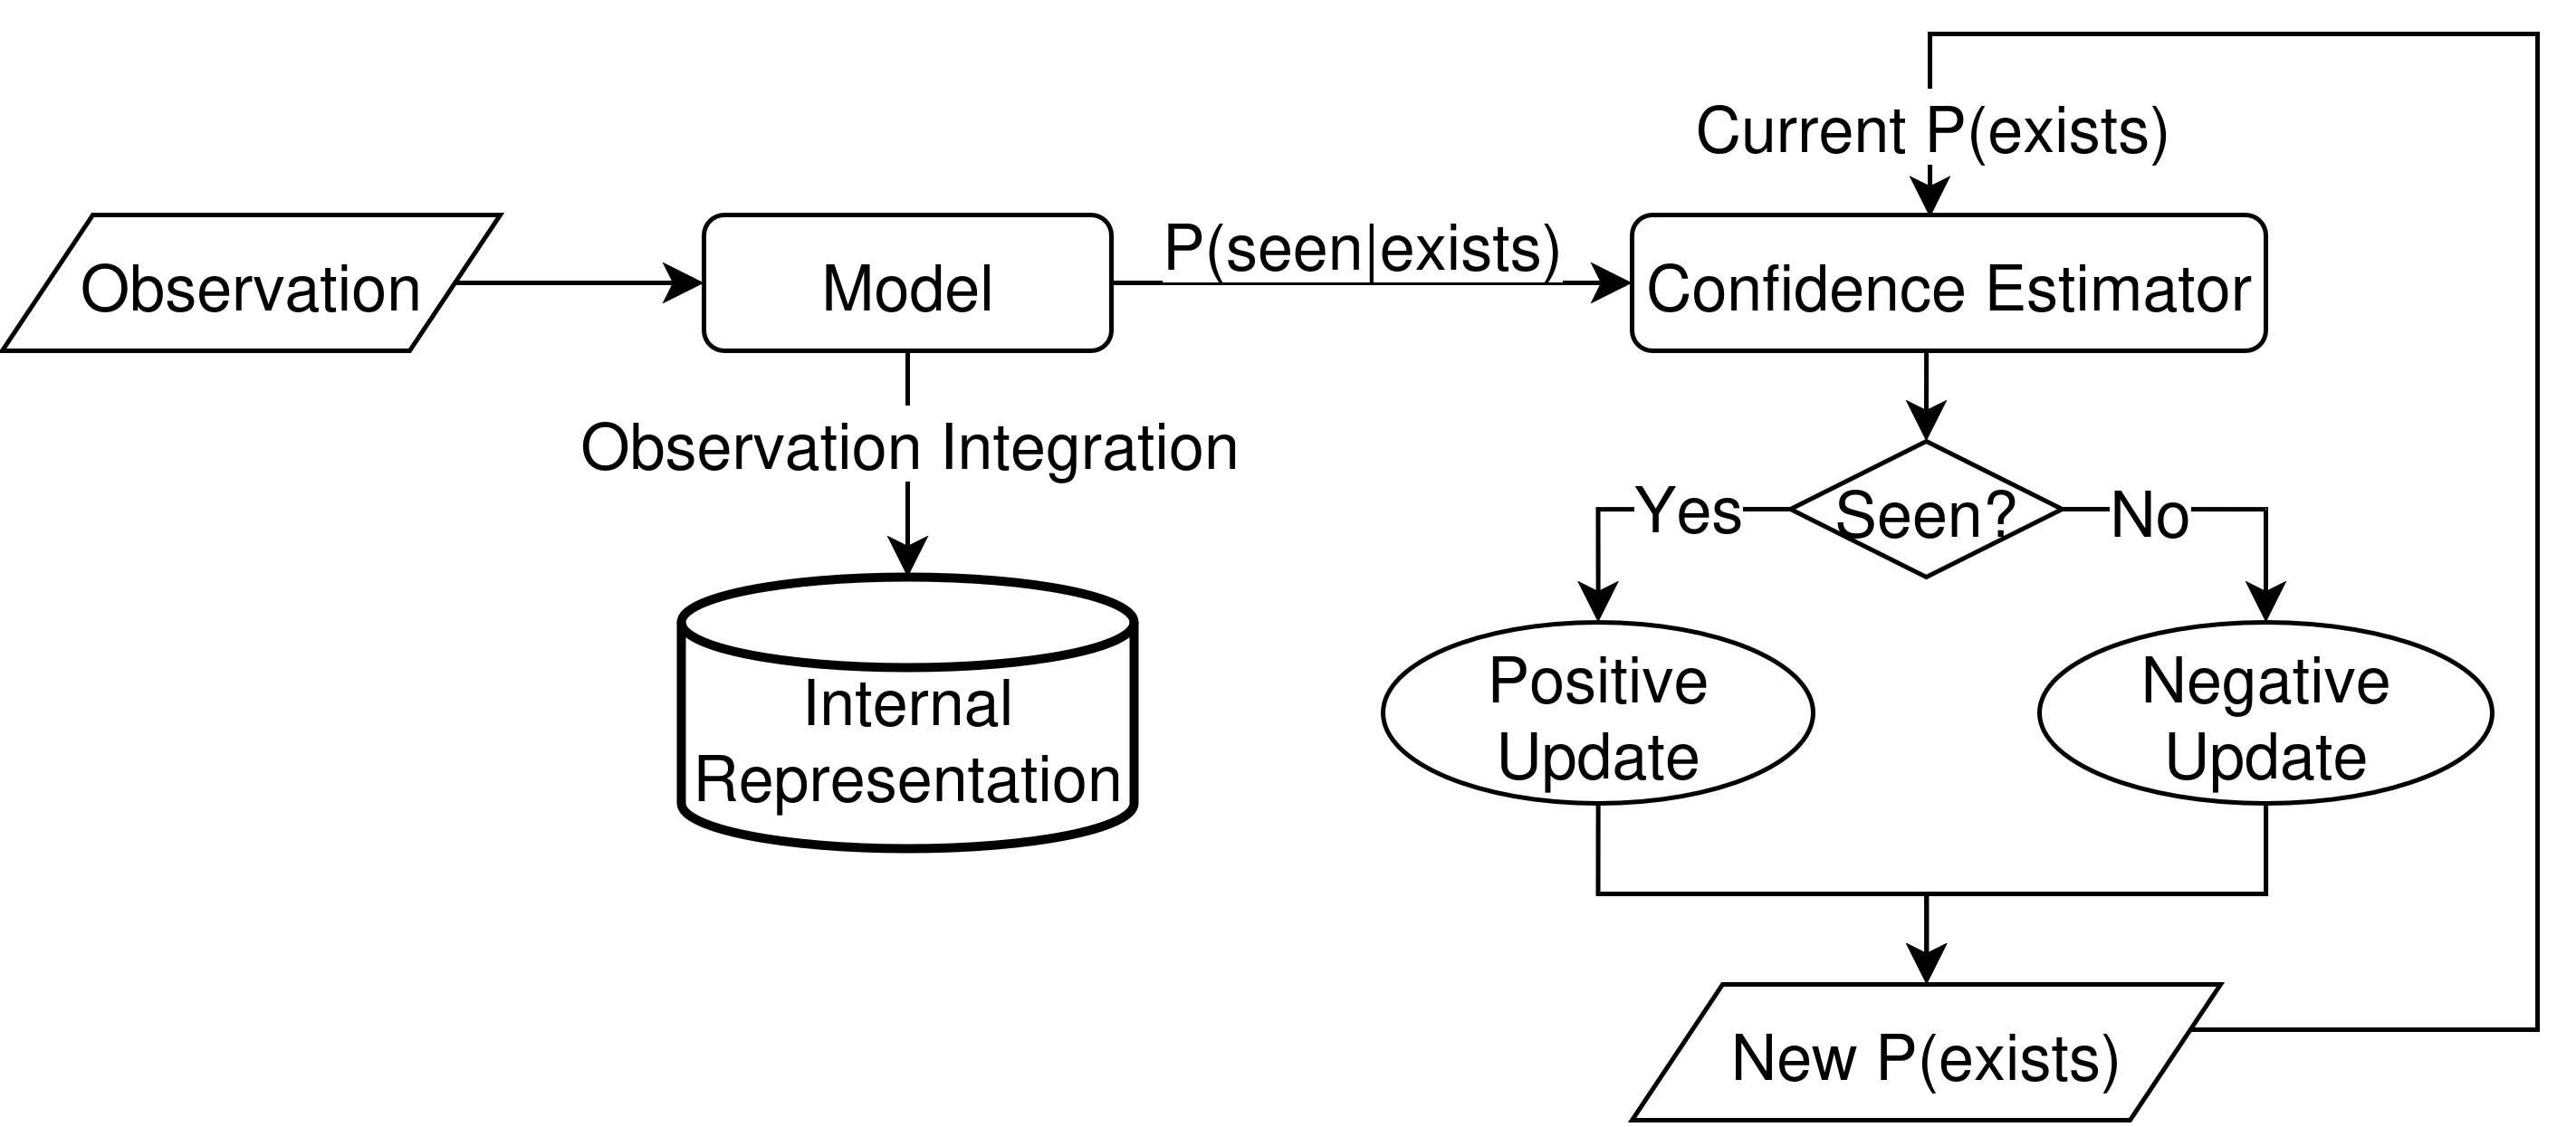
\includegraphics[width=0.7\textwidth]{resources/existence_estimation_framework.png}
    \caption[Existence Estimation Framework]{A flowchart representing the flow of data through the proposed Existence Estimation Framework.}
    \label{fig:existence_estimation_framework}
\end{figure}

The framework consists of two components: the observability model, and the existence probability updater. The observability model estimates the probability of a point being seen from a given viewpoint $P(S^{\boldsymbol{v}}|E)$, and updates its internal representation to integrate new observations. The existence probability updater performs a Bayesian update of the point's existence probability using the prior existence probability $P(E)$, the model estimate $P(S^{\boldsymbol{v}}|E)$, and the new observation's outcome $S$ or $\lnot S$. This approach ensures that negative observations from previously highly observable viewpoints impact the existence probability more strongly than those from more uncertain viewpoints.

\subsubsection{The Bayesian Update Step}

The system updates its confidence for a map point's existence based on environmental observations. This update follows Bayes' theorem, and can therefore be implemented to utilize Bayesian statistics. The events of interest are:
\begin{itemize}
    \item $E$: The event that the map point exists
    \item $S^{\boldsymbol{v}}$: The event that the map point is seen from viewpoint $\boldsymbol{v}$
\end{itemize}

where $\boldsymbol{v} = \{\theta,\phi,d\}$, representing azimuth, elevation and distance from the observer to the point respectively. To formalize, our system updates $P(E) = P(E|S^{\boldsymbol{v}})$ given a positive observation, and $P(E) = P(E|\neg S^{\boldsymbol{v}})$ given a negative observation.

Applying Bayes' theorem, the derived update function is
\[
    P(E) = \begin{cases}
        \frac{P(S^{\boldsymbol{v}}|E)P(E)}{P(S^{\boldsymbol{v}})}           & \text{given }S^{\boldsymbol{v}}      \\
        \frac{P(\neg S^{\boldsymbol{v}}|E)P(E)}{P(\neg S^{\boldsymbol{v}})} & \text{given }\neg S^{\boldsymbol{v}}
    \end{cases}
\]

Additionally, the marginal probability $P(S^{\boldsymbol{v}})$ is
$$
    P(S^{\boldsymbol{v}}) = P(S^{\boldsymbol{v}}|E)P(E) + P(S^{\boldsymbol{v}}|\neg E)P(\neg E)
$$

The probability of a false observation of a non-existent map point is small, but non-zero. The probability of a false match increases in low-light and in low texture environments. The value $\varepsilon$ is assigned to represent this probability, and will be experimentally determined in Section \ref{sec:existence_confidence_eval}.
$$
    \varepsilon = P(S^{\boldsymbol{v}}|\neg E) \approx 0
$$

Finally, assuming the existence of a model function $m$ which estimates the probability of observing the point from a given viewpoint $\boldsymbol{v}$
$$
    m(\boldsymbol{v}) \approx P(S^{\boldsymbol{v}}|E)
$$

The update step can be expressed as
\[
    P(E) = \begin{cases}
        \frac{m(\boldsymbol{v})P(E)}{m(\boldsymbol{v})P(E) + \varepsilon(1-P(E))}             & \text{given }S^{\boldsymbol{v}}      \\
        \frac{(1-m(\boldsymbol{v}))P(E)}{(1-m(\boldsymbol{v}))P(E) + (1-\varepsilon)(1-P(E))} & \text{given }\neg S^{\boldsymbol{v}}
    \end{cases}
\]

\subsubsection{The Observability of Map Points}

Map points are conceptualized as static, infinitesimally small points in 3D Euclidean space. Let the observability of a map point $p$ from a viewpoint $\boldsymbol{v} = \{\theta,\phi,d\}\in[0,2\pi)\times\left[-\frac{\pi}{2},\frac{\pi}{2}\right]\times[0,d_{max})$ be represented by the function
$$
    \operatorname{observable}_p : V \to \{0, 1\}
$$
where $\boldsymbol{v} = \{\theta,\phi,d\}$ represents the azimuth, elevation, and distance from the observer to $p$ respectively. This function returns 1 if $p$ is observed from $\boldsymbol{v}$, and 0 if it is not. From this, an observation of point $p$ can be defined as a vector $\boldsymbol{o}_p=\{\boldsymbol{v},observable_p(\boldsymbol{v})\}$, and a set of $n$ observations of $p$ as $\boldsymbol{O}_p=\{\boldsymbol{o}_{p0},\dots,\boldsymbol{o}_{pn}\}$. For illustrative purposes, figures in the remainder of this thesis may use a simplified 2D representation of these definitions, where $\boldsymbol{v}^{2D}=\{\theta,d\}$. Figure \ref{fig:global_observability_p} shows such a plot representing the global observability of a map point $p$, and the effects of obstructions on observability.

\begin{figure}[!ht]
    \centering
    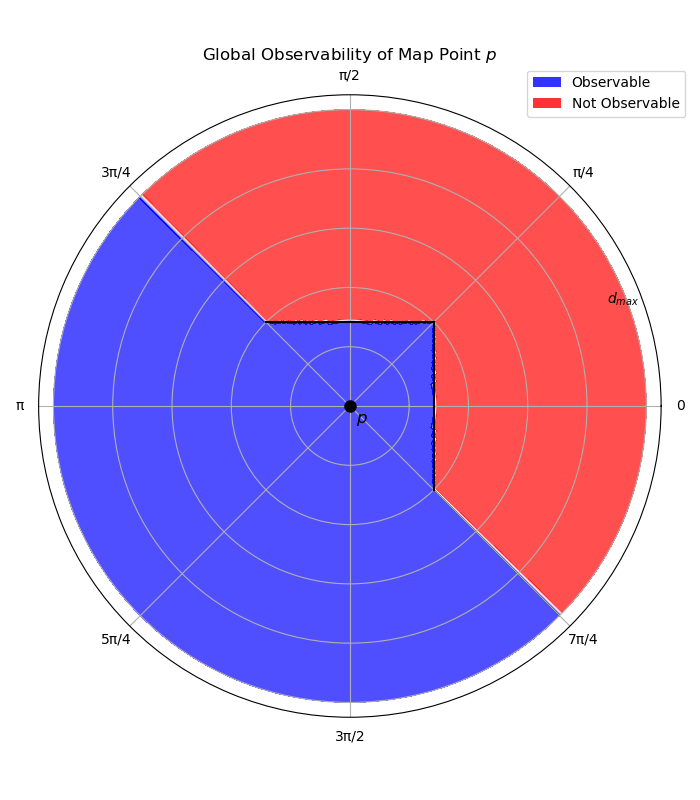
\includegraphics[width=0.7\textwidth]{resources/global_observability_p.png}
    \caption[2D Global Observability]{A 2D representation of the global observability of a map point $p$ near two orthogonal obstructions.}
    \label{fig:global_observability_p}
\end{figure}

The generation of such a plot would require the generation and storage of infinite observations taken from across the domain of viewpoints. The objectives defined in Section \ref{sec:objectives} state that the model's size should be constant and small. Therefore, the models described below must operate either on some fixed, finite number of observations, or on a constant sizes set of metadata.

\subsubsection{Observability Modeling}

The observability model performs two functions: estimation of the probability of the map point being seen from a given viewpoint, and the integration of new observations into its internal representation. The estimation function $\operatorname{m}_p$ takes a viewpoint as an argument, and returns the model's estimate of $P(S^{\boldsymbol{v}}|E)$. The update function takes an observation as an argument, and returns nothing. The goal of any model implementation is to minimize the objective function
$$
    \int |\operatorname{m}_p(\boldsymbol{v}) - \operatorname{observable}_p(\boldsymbol{v})| \,dV
$$
representing the total error between the model's estimate, and the true observability of a point $p$.

\paragraph{K-Nearest Neighbors Model}

A simple method for modeling the observability is the use of a K-nearest-neighbors clustering method. In this model, the estimation is the number of positive observations in the k-nearest observations divided by k. The replacement strategy utilizes feedback from the existence estimator, replacing the nearest observation with the new observation if $\Delta P(E) > \tau$
\paragraph{Binned Model}
\paragraph{Continuous Model}

\subsubsection{Overall Observability}

The models described above are lacking one critical component. Currently, if a model's estimation function returns 1, it is stating that it is fully confident that if the map point exists, it will be seen from the given viewpoint. Therefore, a single negative observation of a point which has always been observable would immediately drop $P(E)$ to zero. To combat this, a damping factor $\delta \in [0,1]$ could be added such that
\[
    P(E) = \begin{cases}
        \delta \frac{m(\boldsymbol{v})P(E)}{m(\boldsymbol{v})P(E) + \varepsilon(1-P(E))}             & \text{given }S^{\boldsymbol{v}}      \\
        \delta \frac{(1-m(\boldsymbol{v}))P(E)}{(1-m(\boldsymbol{v}))P(E) + (1-\varepsilon)(1-P(E))} & \text{given }\neg S^{\boldsymbol{v}}
    \end{cases}
\]
allowing the maximum impact of new observations to be tuned through careful selection of $\delta$. However, this fails to account for the overall observability of the map point. Consider the case shown in Figure \ref{fig:overall_observability}. Clearly, a negative observation within the observable region of the left plot should have a smaller impact on $P(E)$ than a negative observation within the observable region of the right plot.

\begin{figure}[!ht]
    \centering
    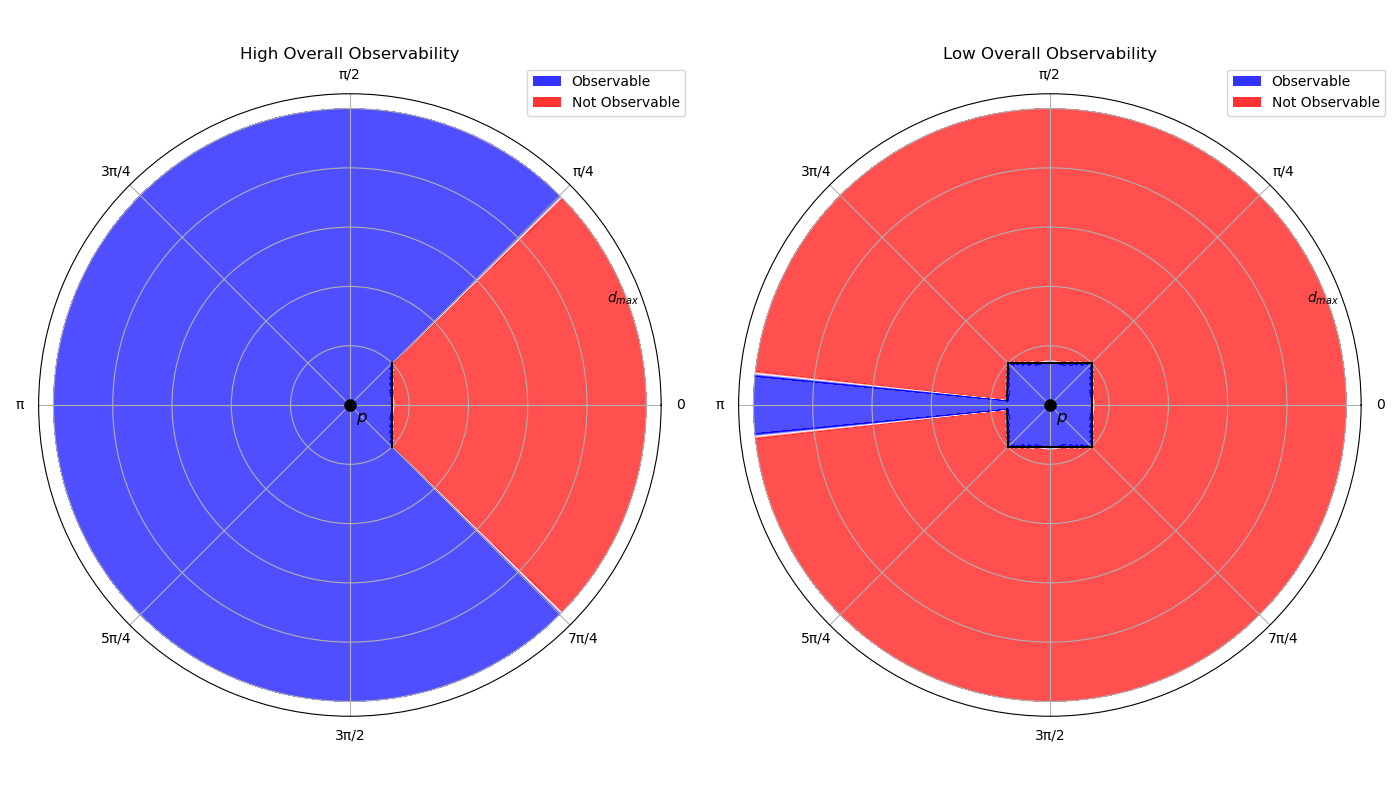
\includegraphics[width=0.9\textwidth]{resources/overall_observability.png}
    \caption[Overall Observability]{A 2D representation of the global observability of a map point $p$ with high overall observability (left) and low overall observability (right).}
    \label{fig:overall_observability}
\end{figure}

Overall observability represents the proportion of viewpoints from which the map point is observable to the total number of viewpoints.